\chapter{Tanulásmenedzsment rendszerek erőforrásigényei}

Minden informatikai rendszernek van erőforrásigénye, vagyis az a minimális hardver konfiguráció, amelyen a rendszer bizonyos számú kéréseket ki tud szolgálni adott időn belül. Az erőforrások mérete befolyásolja a kiszolgálható kérések számát. Ha a kérések száma növekszik akkor növekedhet az erőforrásigény is. A kiszolgálandó kérések típusától, fajtájától függ, hogy pontosan milyen erőforrásokra van igény.
Egy informatikai rendszer esetében a leggyakrabban emlegetett, figyelt, használt erőforrások:
\begin{sajat_itemize}
\item CPU (pl. mennyi processzor időt használ a rendszer, mennyit az alkalmazás),
\item memória (pl. mennyi memóriát használ az alkalmazásunk),
\item tárhely (pl. mennyi tárhely áll rendelkezésünkre),
\item hálózat (pl. mennyire van kihasználva a sávszélesség, mennyi a ki és be irányú forgalom),
\item stb.
\end{sajat_itemize}

\section{Alapvető igények}

\subsection{Az operációs rendszer igényei}
Egy informatikai rendszer teljes erőforrásigénye sok részletből tevődhet össze. Alapvetően meghatározza az operációs rendszer igénye, az erre épülő szolgáltatások (adatbázis szerver, webszerver, levelezőszerver, egyebek) és a főszolgáltatás platformja.
A ma használatos szerver operációs rendszerek alapkövetelményének számít \cite{ws2008sr,ubuntuminhr,redhatcaplim}:

\begin{sajat_itemize}
\item min. 1-1,5 GHz-es CPU (x86 vagy x64), de 2 GHz az ajánlott,
\item min. 512 MB memória, de 2 GB ajánlott \footnote{Red Hat Linux esetében pl. 1 GB/processzor egység},
\item min. 10 GB tárkapacitás.
\end{sajat_itemize}

Gyakran ajánlják a szerverek operációs rendszerének a Linux rendszereket, mivel ezek köztudottan kevesebb memóriát használnak fel, így több marad a többi szolgáltatás számára. 

\subsection{Eltérő platformok, eltérő igények}
Nem csak az LMS-ek, de minden webes alkalmazás esetén is különböző platformokat találunk az alkalmazás szerver oldalán. Az igen elterjedt, középkategóriás PHP mellett az üzleti életben gyakran Java alapokon fejlesztenek, de nem szabad megfeledkezni a .NET-es, Ruby on rails-es, vagy a Python-os megvalósításokról sem. Az egyes platformok különböznek teljesítményükben, ''gyorsaságukban'', megbízhatóságukban és erőforrásigényükben is.

Az egyik legelterjedtebb webes alkalmazás platform a PHP, mivel ez a nyelv szinte minden operációs rendszeren, szinte minden webszerverrel együtt tud működni, és emellett igen jól skálázható.

\subsection{Webszerverek erőforrásigénye}

Ahhoz, hogy el tudjunk indulni a webszerverek erőforrásigényeinek vizsgálatában először meg kell értenünk, hogyan is működnek ezek az alkalmazások. Egy webszerver általában egy többfolyamatos (\angolul{multi-process}) vagy többszálas (\angolul{multi-threaded}) modell szerint működik.\cite{Lu:2001:FCA:882481.883781} Ezek a feldolgozó folyamatok, vagy szálak igény esetén jönnek létre, vagy egy tárolóban előre létrehozott számban várják a beérkező TCP kapcsolatokat, hogy kiszolgálhassák azokat. A széleskörűen használt Apache webszerver a többfolyamatos, készletes modellt alkalmazza.

A HTTP 1.0 esetében minden egyes kérés egy TCP kapcsolatot jelentett, amely így nagyszámú konkurens kapcsolatot igényelt. Ezen javítva a HTTP 1.1-es verziójában megjelent a perzisztens kapcsolat, amely lehetővé teszi, hogy egy kapcsolatba több kérés is belekerüljön.

Ezek a perzisztens kapcsolatok egy új típusú szűk keresztmetszetet hoztak be a szerverekbe. Amióta a kiszolgáló folyamat egy perzisztens kapcsolathoz köthető a CPU kihasználtsága nagyon alacsony. Ezen alacsony kihasználtságon a végrehajtó folyamatok számának növelésével segíthetünk, ám ekkor a virtuális memória kezdhet el vergődni (\angolul{thrashing}). Ezt csak viszonylag sok elérhető memóriával orvosolhatjuk. Ebből következik, hogy a webszerverek inkább memória-, mint processzorigényesek. 

\subsection{Adatbázisszerverek erőforrásigénye}

\todo{adatbázisok igénye MySQL vs. PostgreSQL vs. Oracle vs. MSSQL}

\section{Egy példarendszer: a Moodle}
A Moodle hardveres erőforrásigényei a következők:
\begin{sajat_itemize}
\item min. 160 MB tárolókapacitás (csak a rendszernek \footnote{A teljes tárolókapacitás függ az oktatási anyag mennyiségétől, méretétől, típusától (pl. oktatóvideók)}),
\item min. 256 MB memóriakapacitás (1 GB ajánlott).
\end{sajat_itemize}
Érdemes megjegyezni, hogy a hivatalos Moodle oldalon 1 GB memóriát ajánlanak 50 felhasználó egyszerre történő kiszolgálásához.
Természetesen ez még nem a teljes rendszer igénye, hiszen a webkiszolgálónak és az adatbázisszervernek is van erőforrásigénye \cite{moodleinst}.

A processzor oldaláról nincs különösebb megkötés, a manapság már általánosnak mondható kétmagos, 1,5 GHz-es processzor már elégnek bizonyulhat a rendszer működéséhez.

\section{Igények terhelésváltozások esetén}

\subsection{Terhelésváltozások okozói LMS-eknél}

Az LMS-ek esetében a terhelés változások okozói elsősorban maguk a felhasználók, hiszen ők azok, akik időszakosan megnövekedett kérésszámot intézhetnek a rendszerünk felé. Érdemes lehet ezeket az időszakokat és a hozzájuk kapcsolódó viselkedési változásokat összegyűjteni.

Egy LMS életében a következő erőforrás igényes időszakokat különböztethetjük meg:
\begin{sajat_itemize}
\item kurzus-/vizsgajelentkezési időszak,
\item kurzussal kapcsolatos feladatok beadási határideje,
\item kurzus online teszt, vagy vizsga kitöltés (határ)ideje,
\item egyéb a kurzussal kapcsolatos offline számonkérés,
\item online előadás közvetítés,
\item audiovizuális tananyagokkal rendelkező kurzus számonkérésének ideje, 
\end{sajat_itemize}
és még hosszasan sorolhatnánk.

A következőekben megpróbálom összefoglalni, hogy ezek közül melyik milyen módon terheli meg a rendszerünk erőforrásai.

\subsubsection{Kurzus-/vizsgajelentkezési időszak\protect\footnote{Ezt az alfejezetet a BME KTH Neptun Üzemeltetés által kiadott tájékoztatók alapján írtam, amelyeket a rendszer bejelentkező oldalán, a "Letölthető dokumentumok" résznél találhatóak.}}

Sajnos a BME hallgatóinak nem ismeretlen a Neptun Egységes Tanulmányi Rendszer vizsga- és tárgyjelentkezési időszakokban történő kiesése. Ezekben az időszakokban rohamosan megnő az egyszerre aktív felhasználók száma, amivel a rendszer nem tud megbirkózni. Az üzemeltetés mindent megtesz annak érdekében, hogy a rendszer működőképes legyen a több ezer felhasználó esetén is, de ha valamelyik rétegben egy-egy erőforrás nem tudja feldolgozni a kéréseket, akkor az az egész rendszerre kihatással van.

A rendszer terhelés elosztását egy virtualizált gépre telepített szoftver végzi. A 2011. év januári tárgyfelvételi időszakában ez az ingyenes, de több helyen sikerrel alkalmazott szoftver 4000-5000 konkurens felhasználót még ki tudott szolgálni, de az efölötti kérésekkel tömegével már nem volt képes megbirkózni.

A rendszer úgy van kialakítva, hogy a terheléselosztó építi ki a kapcsolatot a webszerverekkel, viszont amikor az összeomlik a már felépített kapcsolatok is elvesznek. A felhasználók ebből annyit tapasztaltak, hogy a rendszer csak hosszú idő után engedte őket belépni a rendszerbe, majd ezután gyakran ki is dobta őket.

A felhasználók a negatív tapasztalatokra még agresszívebben próbálták elérni a rendszert (folyamatos oldallekérések, frissítések), amely viselkedés csak növelte a kiszolgálatlan kérések számát. Mindeközben a webszerverek, és az adatbázis szerverek kihasználtsága a nullához közelített, hiszen a terheléselosztó nem   volt képes a kéréseket továbbítani feléjük.

A Neptun rendszer a júniusi tárgyfelvételi időszakot is zökkenővel viselte. A június 7-én 18 órakor kezdődő felhasználói rohamot, ami 6000 egyidejű, aktív felhasználót jelentett ezúttal a terheléselosztó jól viselte, ám pontosan emiatt az adatbázisszerver nem tudod megküzdeni a nagy számú kéréssel, és megtelt a memóriája.

Ennek következtében az üzemeltetésnek le kellett állítani az egész rendszert, újra konfigurálni az adatbázis szervert (szerencsére mivel virtualizált, felhő alapú rendszerről beszélünk ezért viszonylag egyszerűen megnövelni a memóriáját), majd újraindítani azt, és a webszervereket. Ezután a rendszer már megfelelően működött, alig 10 perc leforgása alatt 6000 felhasználó tudott belépni, és 22500 tárgyat felvenni.

A 2011. augusztus végi tárgyfelvételi időszak jól jellemzi, hogy mennyire függ egy ilyen rendszer a felhasználói viselkedéstől.  Mivel a hallgatóknak már lehetőségük volt a nyár elején felvenni a következő féléves tárgyaikat, ezért a véglegesítési időszakban elmaradt a szokásos terhelés.

A 2011. november 28-án 18 órakor kezdődő vizsgajelentkezés során megint problémák voltak a rendszerrel. Ezúttal a terheléselosztó és a webszerverek tökéletesen működtek, azonban az adatbázis szerver két rendszerparaméter miatt újraösszeomlott. A szerver újrakonfigurálásával, és a rendszer teljes újraindításával a problémát elhárították, és a felhasználók újra megrohanhatták a Neptunt.

A történtek tanulsága, hogy egy ilyen összetett infrastruktúra esetében elég az egyik rétegben bekövetkező hiba, és az az egész rendszerre hatással lehet. Az üzemeltetés automatizált terheléstesztekkel próbálta megkeresni a rendszer szűk keresztmetszetét, és új konfigurációs beállításokkal megszüntetni azokat, de a felhasználói viselkedést nem tudták egyik esetben sem előre meghatározni.

\Aref{tab:neptunusers}.~táblázatban látható, hogy az adott időszakokban hogyan alakult a konkurens felhasználók maximális száma (\textit{Max. felhasználó}) és a rendszer által még kiszolgálható felhasználók száma (\textit{Op. felhasználó}). (Forrás: a BME KTH Neptun Üzemeltetés által kiadott tájékoztatók)

\begin{table}[h]
	\caption{A Neptun rendszer konkurens felhasználóinak száma}
	\centering
	\small
	\begin{tabular}{| p{3.0cm} | p{2.0cm} | p{3.0cm} | p{3.0cm} |}
		\hline
		\rowcolor{MyTableColor} \textbf{Dátum} & \textbf{Jelleg} & \textbf{Max. felhasználó} & \textbf{Op. felhasználó} \\
		\hline
		2010.11.29. 18:00 & vizsga & 7303 & 4623 \\
		\hline
		2010.12.22. 06:00 & tárgy (EO) & 831 & 831 \\
		\hline
		2011.01.10. 18:00 & tárgy & 12062 & 4837 \\
		\hline
		2011.01.12. 18:00 & tárgy (EP) & 1765 & 1765 \\
		\hline
		2011.01.31. 16:00 & tárgy & 1519 & 1519 \\
		\hline
		2011.05.02. 18:00 & vizsga & 2761 & 2761 \\
		\hline
		2011.06.07. 18:00 & tárgy & 6095 & 6095 \\
		\hline
		2011.08.29. 16:00 & tárgy & 1247 & 1247 \\
		\hline
		2011.11.28. 18:00 & vizsga & 4897 & 4897 \\
		\hline
	\end{tabular}
	\normalsize
	\label{tab:neptunusers}
\end{table}


\Aref{fig:neptun_003}.~ábrán látható a 2011. június havi tárgyfelvételi időszak néhány jellemző tárgyfelvétellel kapcsolatos adata. Jól megfigyelhető, hogy az első órában milyen alacsony a sikeres tárgyfelvételek száma, hiszen ebben az időszakban a rendszer nem üzemelt megfelelően, majd a következő oszlopban a már újra konfigurált és újraindított rendszer teljesítménye/felhasználói aktivitása látható.

\begin{figure}[!ht]
\centering
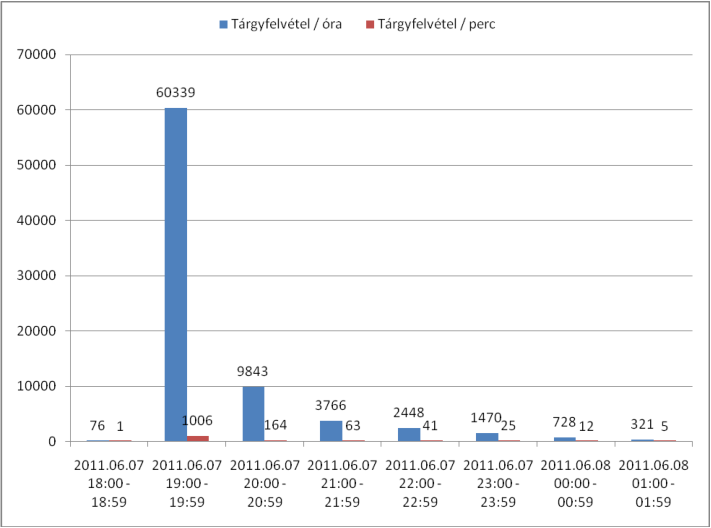
\includegraphics[width=100mm, keepaspectratio]{figures/neptun_003.png}
\caption{Tárgyfelvételek száma a Neptun rendszerben (Forrás: a BME KTH Neptun Üzemeltetés által kiadott tájékoztatók)}
\label{fig:neptun_003}
\end{figure}

A 2011. augusztus végig időszakot \aref{fig:neptun_004}.~ábra mutatja be. Mivel ekkor a rendszer nem volt annyira leterhelve, ezért itt az első oszlop a legmagasabb, majd a másodikban hirtelen csökkenés következett be, végül az idő folyamán fokozatosan csökkent a terhelés.

\begin{figure}[!ht]
\centering
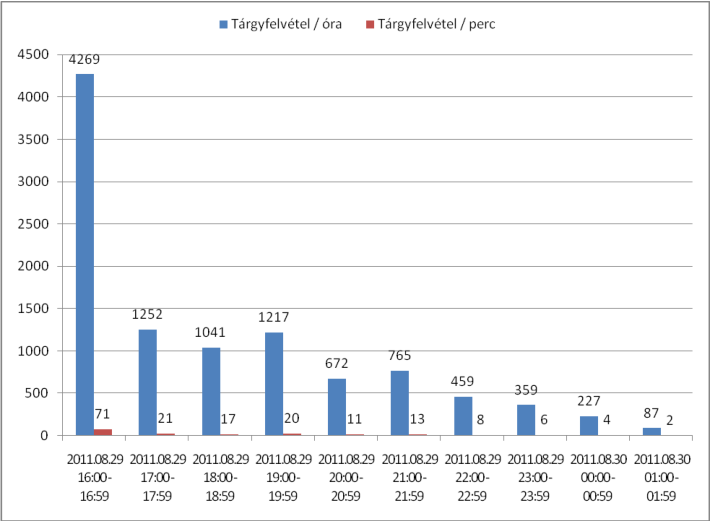
\includegraphics[width=100mm, keepaspectratio]{figures/neptun_004.png}
\caption{Tárgyfelvételek száma a Neptun rendszerben (Forrás: a BME KTH Neptun Üzemeltetés által kiadott tájékoztatók)}
\label{fig:neptun_004}
\end{figure}

\Aref{fig:neptun_005}.~ábrán a 2011. novemberi tárgyfelvétellel kapcsolatos adatokat láthatjuk. A rendszer kezdeti működési nehézségei itt is jól kivehetők.

\begin{figure}[!ht]
\centering
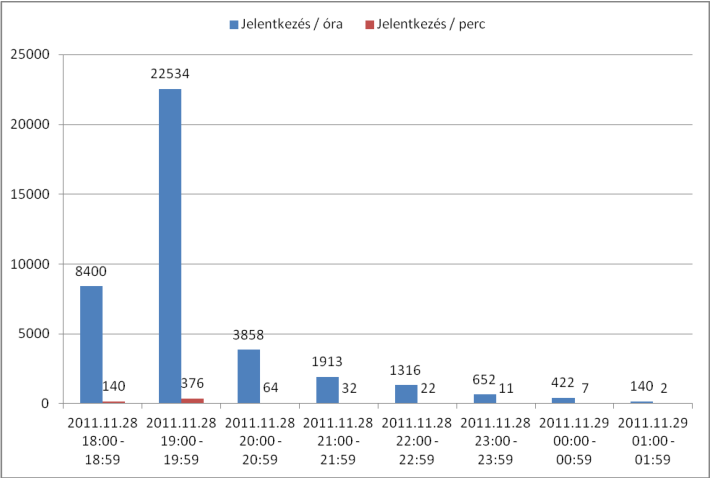
\includegraphics[width=100mm, keepaspectratio]{figures/neptun_005.png}
\caption{Tárgyfelvételek száma a Neptun rendszerben (Forrás: a BME KTH Neptun Üzemeltetés által kiadott tájékoztatók)}
\label{fig:neptun_005}
\end{figure}

\subsubsection{Kurzussal kapcsolatos feladatok beadási határideje}

Hallgatók jellemző viselkedése, hogy megpróbálják az utolsó pillanatban elkészíteni a kiadott feladatokat, amelynek következtében a határidő előtti rövid időintervallumban megnövekszik a rendszerben egyszerre tartózkodó felhasználók száma, és állományok feltöltésével esetlegesen túlterhelik a rendszer hálózatát, adatbázisát és nem előrelátó üzemeltetés esetén a tárhely szabad helyének méretében is kritikus szintet érhetnek el.

\subsubsection{Kurzus online teszt, vagy vizsga kitöltés (határ)ideje}

Egy oktatási rendszerben meglehet határozni olyan időintervallumokat, amelyek egy kurzus tesztjének kitöltésére engedélyezett időszak. A tesztet az intervallum elejétől a végéig lehetséges kitölteni, azon kívül a teszt kitöltése letiltott funkció. Ezzel a felhasználók arra vannak kényszerítve, hogy az adott intervallumon belül bejelentkezzenek a rendszerbe, és kitöltsék a megadott tesztet.

Mivel az időintervallum meghatározott (az üzemeltetés is könnyen tudomást szerezhet róla), és a várható felhasználói létszám is ismert (az adott kurzuson résztvevő felhasználók száma a maximum), azért viszonylag jól fel lehet készülni erre az erőforrással kapcsolatos igényváltozásra. Természetesen itt sem tudjuk 100\%-osan meghatározni, hogy melyik időpillanatban hány felhasználó lesz a rendszerben, és a felhasználó viselkedéstől is nagyban függ az eloszlás, de maximális értékeket meghatározhatunk. Persze nem biztos, hogy ez költség szempontjából az optimális megoldás.

\subsubsection{Egyéb a kurzussal kapcsolatos offline számonkérés}

Napjainkban egyre több oktatási anyag kerül fel online tárhelyre, amelyet az LMS-ek alapból támogatnak. Egy-egy számonkérés előtt megnövekedhet ezen oktatási anyagok letöltésének száma, amely az anyag méretétől, számától és a kurzusra jelentkezett felhasználók számától függően terhelheti az adatbázist és a hálózatot.

Ebben az esetben a feltöltésekhez hasonlóan nem lehetséges biztos modellt alkotni az erődforrásigények változásáról, hiszen itt is nagyban függünk a felhasználói viselkedéstől. Míg folyamatosan készülő diákok az egész félévben elosztott terhelést jelentenek, addig az utolsó pillanatosok a számonkérés előtt nem sokkal terhelhetik a rendszert. 

\subsubsection{Online előadás közvetítés}

Az Internet térnyerésével, és a széles sávú kapcsolatok terjedésével megjelent az \angolul{online stream} lehetősége. Egy ilyen közvetítés egy bizonyos időintervallumban terhelheti a hálózatunkat. Az elérhetőségének korlátozásával (pl. csak az adott kurzust felvett felhasználók nézhetik) a maximális nézőszámot is meg tudjuk előre határozni. Tehát összességében egy ilyen eseményre viszonylag jól fel tudjuk készíteni a rendszerünket erőforrások szempontjából.  

\subsubsection{Audiovizuális tananyagokkal rendelkező kurzus számonkérésének ideje}

Ez az eset az online közvetítés és a számonkérések egyvelege. Mivel a számonkérés ideje rögzített, így addig az időpontig számíthatunk arra, hogy a rendszerünket az adott kurzus felhasználói terhelni fogják. A terhelés főleg a hálózatot fogja érinteni.

Nagyon eltérő terheléseket kaphatunk attól függően, hogy az oktatási anyag letölthető-e vagy csak online nézhető. Az előbbi esetben nagyobb az esély az időben jobban szétkenődő erőforrásigény növekedésekre, míg az utóbbinál a határidő előtt nagy konkurens felhasználói számmal és igénynövekedéssel kell számolnunk. Ennek oka lehet, hogy az online elérhető anyagot a számonkérés előtt nem sokkal fogják megnézni a felhasználók, amivel a rendszerünket terhelik. Ellenben a letölthető anyag esetében meg van az a lehetőség, hogy néhány felhasználó már jóval a határidő előtt letölti azt, így csökkentve a maximális felhasználók számát a kritikus időpontban.

\section{Modellek}\label{sec:modellek}

\subsection{Modellezési problémák}

Az LMS-ek üzemeltetésének legnagyobb problémája, hogy nem rendelkezünk olyan modellekkel, amelyekkel 100\%-osan előre tudnánk jósolni a rendszer zavartalan működéséhez, az áteresztőképességének szinten tartásához szükséges erőforrások mennyiségét.

A piacon igen sok terhelés tesztelő alkalmazást lehet találni. Ezek közül az egyik legismertebb az Apache JMeter (\href{https://jmeter.apache.org/}{https://jmeter.apache.org/}). Ez egy igen részletesen konfigurálható, elsősorban webes alkalmazások funkcionális terhelés tesztjeire készített asztali alkalmazás.

Valószínűsíthető, hogy a Neptun rendszer üzemeltetése is hasonló szoftverrel próbálta tesztelni az infrastruktúrájának terhelhetőségét, de ahogy láthattuk ez nem vezetett célra. Ezekkel a szoftverekkel meg tudjuk vizsgálni, hogy a rendszerünk mekkora maximális terhelést visel el, de azt már nem tudjuk meghatározni, hogy a való életben mekkora lesz ez az érték. A probléma itt is, mint az informatika sok más területén is, a felhasználó és annak nem előre jelezhető viselkedése.

A Neptun esetében is megfigyelhető, hogy egy kurzus-, vagy tárgyfelvételi időszak kezdetén maximális az aktív felhasználók száma, majd ezután az idő elteltével rohamosan csökken. Általában, hiszen bemutattunk egy olyan esetet is, amikor nem következett be az elvárt roham, mert a felhasználók már korábban elintézhették a tárgyfelvételt, ezért csak az időben szélesen elosztva jelentek meg átlagos értékek a grafikonjainkon, amikor is néhány felhasználó valószínűleg véglegesítette a tárgyait.

Hasonlóan nem teljesen kiszámítható egy kurzus számonkérése előtti felhasználói érdeklődés. Hiszen előfordulhat, hogy két olyan kurzus esetén, amely rendelkezik írásos, és audiovizuális oktatási anyaggal, eltérő módon az egyik kurzus esetében csak az írásos segédanyagot, a másik esetben pedig a multimédiás tartalmat fogják igénybe venni, a rendszer szempontjából ezzel eltérő erőforrás igényeket generálva.

\subsection{Lehetséges modell alkotások}

Az oktatási rendszerek esetében egy lehetséges modell alkotási lehetőség lehet az összegyűjtött monitorozási, naplózási adatok statisztikai elemzése. Ezekkel az adatokkal valamennyire jósolható egy esemény által igényelt erőforrások mennyisége, amelynek segítségével akár proaktívan is be lehet avatkozni a rendszer működésébe.

\Aref{fig:neptun_003}., \ref{fig:neptun_004}. és \ref{fig:neptun_005}.~ábrákon látható grafikonokból is le lehet vonni következtetéseket a felhasználók és a rendszer felé irányuló kérések számának eloszlásáról. Hasonló módon a Munin (\href{http://munin-monitoring.org/}{http://munin-monitoring.org/}) nevű grafikus monitorozó eszközzel megoldható, hogy az LMS egyes eseményeit (pl. aktuális felhasználók, hálózati eszközök kihasználtsága, stb.) grafikonok segítségével jellemezzük. Persze mindezen grafikusan ábrázolt adatoknak csak akkor van értelme, ha mellette azt is tudjuk, hogy az éppen vizsgált időintervallumban milyen oktatással kapcsolatos események történtek (pl. teszt kitöltés, online előadás, stb.). 
